\documentclass[10pt,a4paper,twoside,titlepage,twocolumn]{article}
\usepackage[utf8]{inputenc}
\usepackage[T1]{fontenc}
\usepackage[ngerman]{babel,varioref}
\usepackage[left=0.7cm,right=0.7cm,top=0.7cm,bottom=0.7cm,includeheadfoot]{geometry}

\usepackage{amsmath}
\usepackage{amssymb}
\usepackage{graphicx}
\usepackage{xcolor}
\usepackage{siunitx}



\begin{document}
    \graphicspath{ {./Images/} }


\definecolor{formulablue}{RGB}{219,219,255}
\newcommand{\formula}[1]{\colorbox{formulablue}{#1}}

\newcommand{\unitText}[3]{\noindent\textit{#1} : #2 [#3]}

\definecolor{refrot}{RGB}{183,28,42}
\newcommand{\refskript}[1]{\textcolor{refrot}{Skript S.#1}}



% \titlespacing*{\section}{0pt}{12pt}{0pt}
% \titlespacing*{\subsection}{0pt}{0pt}{0pt}
% \titlespacing*{\subsubsection}{0pt}{0pt}{0pt}


\title{\vspace{50mm}AdvDeLearn \\ [1ex] \large Summary}
\author{Lukas Schöpf}
% \titlepic{\vspace{50mm}\includegraphics[width=0.25\textwidth]{Elvis}}


% Code format
% Define the Gruvbox light colors
\definecolor{gruvbox_bg}{HTML}{fbf1c7}
\definecolor{gruvbox_fg}{HTML}{3c3836}
\definecolor{gruvbox_yellow}{HTML}{d79921}
\definecolor{gruvbox_red}{HTML}{cc241d}
\definecolor{gruvbox_green}{HTML}{98971a}
\definecolor{gruvbox_blue}{HTML}{458588}
\definecolor{gruvbox_purple}{HTML}{b16286}
\definecolor{gruvbox_aqua}{HTML}{689d6a}
\definecolor{gruvbox_orange}{HTML}{d65d0e}


% \lstdefinestyle{cppstyle}{
% 	language=C++,
% 	basicstyle=\ttfamily\footnotesize,
% 	numbers=left,
% 	numberstyle=\tiny,
% 	numbersep=5pt,
% 	tabsize=4,
% 	showspaces=false,
% 	showstringspaces=false,
% 	frame=single,
% 	rulecolor=\color{gruvbox_fg},
% 	backgroundcolor=\color{white},
% 	keywordstyle=\color{gruvbox_orange},
% 	commentstyle=\color{gruvbox_aqua},
% 	stringstyle=\color{gruvbox_green},
% 	identifierstyle=\color{gruvbox_fg},
% 	emphstyle=\color{gruvbox_red},
% 	emph={int, double, string, cout, TimerHandle_t, BaseType_t, timerPWMPeripheral_t, SemaphoreHandle_t, TaskHandle_t, QueueHandle_t},
% 	xleftmargin=5mm,
% 	xrightmargin=\parindent
% }

	\maketitle
	\setlength\parindent{0pt}

	% Uncomment these lines if you want to include the respective sections
	\section{Deep Learning Recap}

\subsection{Neural Network Types}
\subsubsection{Multi-Layer Perceptron (MLP)}
\begin{itemize}
    \item Input: \( n \)-dimensional, Output: \( m \)-dimensional.
    \item Fully connected hidden layers.
    \item Applications: Classification, regression, feature transformation, and dimensionality reduction.
\end{itemize}
Base equation / shallow network:
\[
f(x) = \sum_{i = 1}^{N} a_i \sigma(\mathbf{w}_i\cdot\mathbf{x} + b_i)
\]
For deep network:
\[
    y = f_3(f_2(f_1(x)))
\]

\subsubsection{Convolutional Neural Networks (CNNs)}
\begin{itemize}
    \item Feature extraction through convolutional layers.
    \item Supports multi-channel inputs (e.g., RGB images).
    \item Applications: Image processing, signal analysis, time-series data, 3D datasets like MRI.
\end{itemize}
Properties:
\begin{itemize}
    \item Weights(parameters) are shared
    \item Connections are sparse
    \item Each node in a layer has a receptive field
\end{itemize}
For multi-channel inputs, a diffrent kernel is applied for each channel.
The resulting channels are summed:
\[
C_{out,j} = b_j + \sum_{k=0}^{C_{in}-1} w \star f(x,y)
\]

Good practiec is to replace large filters with multiple smaller.

\subsection{Key Architectural Patterns}
\subsubsection{Reducing and Increasing Output Size}
\begin{itemize}
    \item Techniques: Strided convolutions, pooling, upsampling, and transposed convolutions.
\end{itemize}

\subsubsection{Improving Efficiency}
\begin{itemize}
    \item Bottleneck layers: Use \( 1 \times 1 \) convolutions to reduce channel dimensions.
    \item Separable filtes(for $7\times7$ use $(7\times1) \cdot (1\times7)$).
    \item Depthwise separable convolutions for sparse connectivity.
    \item Instead of one $11 \times 11$ conv. layer use 5 $3\times3$.
\end{itemize}

\subsubsection{Residual Connections}
\begin{itemize}
    \item Allow better gradient flow in deep networks.
    \item Key to ResNet architectures.
\end{itemize}

\subsubsection{Regularization}
\begin{itemize}
    \item Techniques: Dropout, \( L_2 \)-regularization.
    \item Goal: Prevent overfitting and improve generalization.
\end{itemize}

\subsection{Training Considerations}
\subsubsection{Layer/Batch normalization}
\begin{itemize}
    \item Use to normalize input to layers
    \item Accelerates training, importves generalization
\end{itemize}
\begin{equation*}
    \hat{x}^{(i)} = \frac{x^{(i)} - \mu_{\text{batch}}}{\sqrt{\sigma^2_{\text{batch}} + \epsilon}}
\end{equation*}
    
\begin{equation*}
    y^{(i)} = \gamma \hat{x}^{(i)} + \beta
\end{equation*}
\(\gamma\) and \(\beta\) are learnd from mini batches.

\subsubsection{Weight Initialization}
\begin{itemize}
    \item Xavier initialization ensures variance proportionality.
\end{itemize}

\subsubsection{Activation Functions}
\begin{itemize}
    \item Options: ReLU, Leaky ReLU, Sigmoid, Tanh, etc.
    \item ReLU variants preferred for stability.
\end{itemize}

\subsubsection{Optimizers}
\begin{itemize}
    \item Popular choices: SGD, Adam, RMSprop.
    \item Trade-offs between convergence speed and generalization.
\end{itemize}


	\section{Attention and Transformers}
\begin{figure}[ht]
    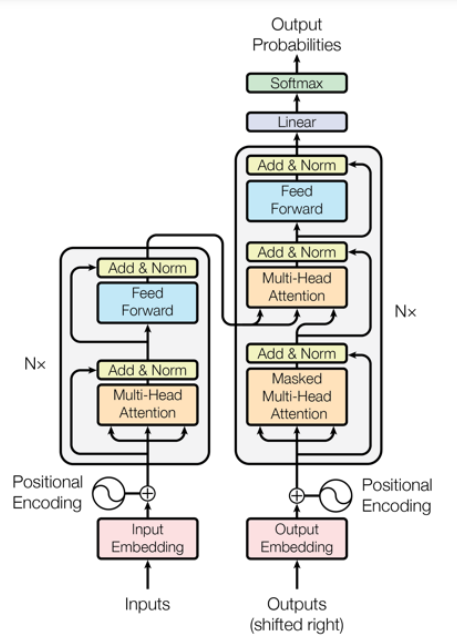
\includegraphics[width=0.6\columnwidth]{figures/AttentionTransformer/Transformer.png}
\end{figure}
\subsection{Sequence Processing}
\subsubsection{Recurrent Neural Networks (RNNs)}
\begin{itemize}
    \item Process sequences using recurrent cells with an internal state \( h \).
    \item Computation at each time step:
    \[
    h_t = \sigma(W_{hh} h_{t-1} + W_{xh} x_t + b_h)
    \]
    \item Output:
    \[
    y_t = W_{hy} h_t + b_y
    \]
    \item Common challenges: vanishing and exploding gradients.
\end{itemize}

\subsubsection{Advanced RNN Variants}
\begin{itemize}
    \item LSTMs handle long-term dependencies using gates:
    \[
    c_t = f_t \odot c_{t-1} + i_t \odot \tanh(W_c x_t + U_c h_{t-1} + b_c)
    \]
    \[
    h_t = o_t \odot \tanh(c_t)
    \]
    \item \(c_t\) long term memory
    \item \(h_t\) short term /working memory
    \item GRUs simplify LSTMs by merging the forget and input gates:
    \[
    h_t = (1 - z_t) \odot h_{t-1} + z_t \odot \tilde{h}_t
    \]
\end{itemize}
\begin{figure}
    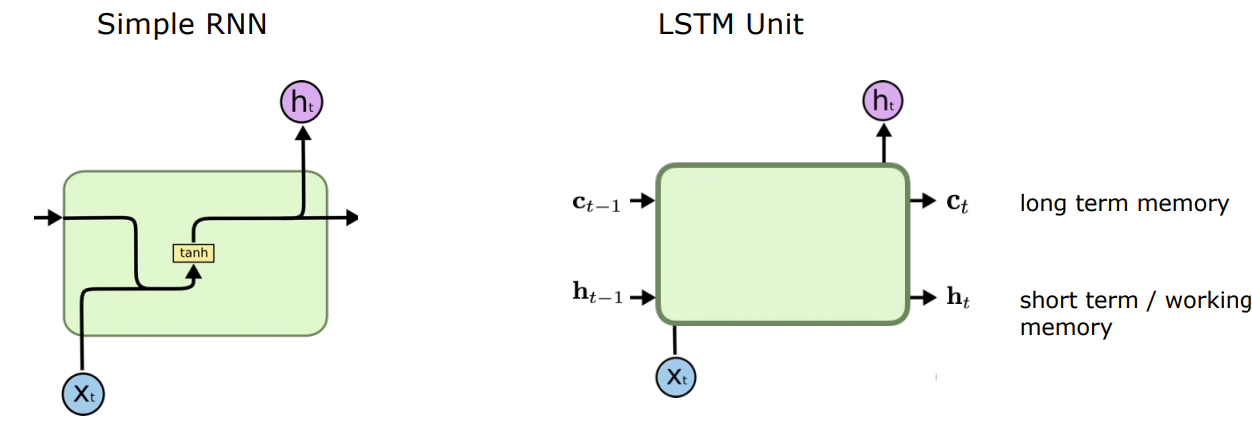
\includegraphics[width= \columnwidth]{figures/AttentionTransformer/RNNLSTM.png}
\end{figure}
\subsection{Attention Mechanism}
\subsubsection{Concept and Applications}
\begin{itemize}
    \item Attention aligns inputs with outputs for tasks like translation and image captioning.
    \item Improves handling of long sequences and offers interpretability.
\end{itemize}

\subsubsection{Attention Calculation}
\begin{itemize}
    \item Compute attention weights:
    \[
    \text{score}(q, k) = \frac{q \cdot k}{\sqrt{d_k}}
    \]
    \item Normalize weights with softmax:
    \[
    \alpha_{ij} = \frac{\exp(\text{score}(q_i, k_j))}{\sum_{j'} \exp(\text{score}(q_i, k_{j'}))}
    \]
    \item Compute the attention output as a weighted sum of values:
    \[
    \text{Attention}(Q, K, V) = \text{softmax}\left(\frac{QK^\top}{\sqrt{d_k}}\right)V
    \]
\end{itemize}

\subsection{Transformer Architecture}

\subsubsection{Encoder Architecture}
\begin{itemize}
    \item The encoder consists of \( N \) identical layers, each with:
    \begin{enumerate}
        \item Multi-head self-attention:
        \[
        \text{MultiHead}(Q, K, V) = \text{Concat}(\text{head}_1, \ldots, \text{head}_h)W^O
        \]
        where
        \[
        \text{head}_i = \text{Attention}(QW_i^Q, KW_i^K, VW_i^V)
        \]
        \item A feedforward network applied to each position:
        \[
        \text{FFN}(x) = \text{ReLU}(0, xW_1 + b_1)W_2 + b_2
        \]
        \item Residual connections and layer normalization for stability:
        \[
        \text{Output} = \text{LayerNorm}(x + \text{SubLayer}(x))
        \]
    \end{enumerate}
\end{itemize}

\subsubsection{Decoder Architecture}
\begin{itemize}
    \item The decoder mirrors the encoder but includes an additional sub-layer for cross-attention:
    \begin{enumerate}
        \item Masked multi-head self-attention:
        \[
        \text{Attention}(Q, K, V) = \text{softmax}\left(\frac{QK^\top}{\sqrt{d_k}}\right)V
        \]
        Masking prevents the decoder from seeing future tokens during training.
        \item Cross-attention, where queries come from the decoder, and keys/values come from the encoder.
        \item Feedforward network and residual connections (as in the encoder).
    \end{enumerate}
    \item A final linear layer projects the decoder's output to the vocabulary size, followed by a softmax:
    \[
    p(y_t | y_{<t}, x) = \text{softmax}(W_s h_t + b_s)
    \]
\end{itemize}

\subsubsection{Positional Encoding}
\begin{itemize}
    \item Adds sequence order information:
    \[
    PE_{\text{pos}, 2i} = \sin\left(\frac{\text{pos}}{10000^{2i/d_{\text{model}}}}\right)
    \]
    \[
    PE_{\text{pos}, 2i+1} = \cos\left(\frac{\text{pos}}{10000^{2i/d_{\text{model}}}}\right)
    \]
\end{itemize}
	\section{Vision Transformer (ViT)}
\begin{figure}[]
    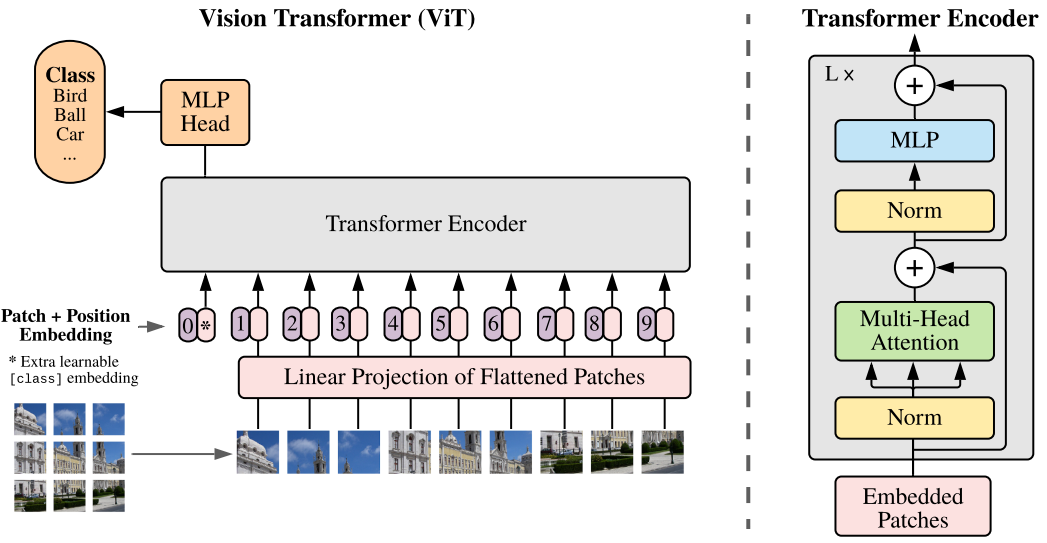
\includegraphics[width=\columnwidth]{figures/VisionTransformer/ViT.png}
\end{figure}
\begin{itemize}
    \item Extract square Images Patches
    \item Flatten Patches and project them to the embedding dimension D
    \item These embeddings are input to the Transformer
    \item Output of Transformer is fed into MLP or a singel layer
    \item Position embeddings added to input embeddings
\end{itemize}

Excellent results when pretrained on larger dataset(14M-300M)images and fine-tuned.

\subsection{Vertical Design}
\begin{figure}[!h]
    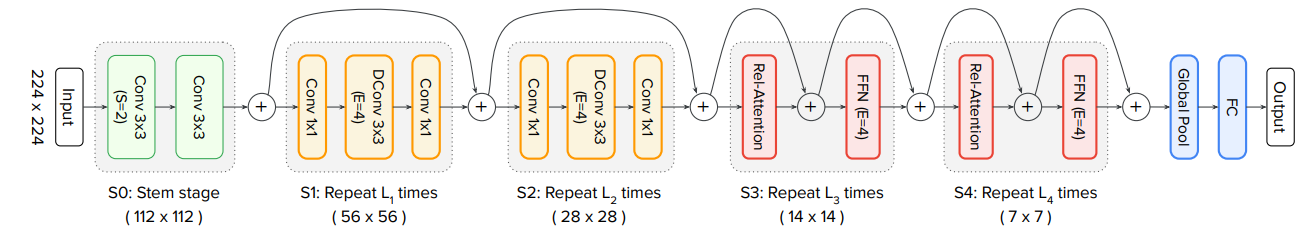
\includegraphics[width=\columnwidth]{figures/VisionTransformer/verticalDesign.png}
\end{figure}
\begin{itemize}
    \item Applying the relative-attention at pixel level is Computationally not possible
    \item A down-sampling of the image is needed
    \item Mimics CNNs architecture
\end{itemize}
\subsection{Relative self-Attention}
\begin{itemize}
    \item Combines Convolution and Attention
    \item Considers realitve position of tokens by introducing a global kernel value \(w_{i-j}\)
    \item  \textbf{Formula!}
\end{itemize}
	\section{Kolmogorov-Arnold Networks (KAN)}
The idea is to better approximate smooth functions with B-splines.

\subsection{B-Splines}
B-Splines are recursivly defined over a local area of knots(x coordinates)
Defined as \(B_{x-position,order}\).
\begin{figure}
    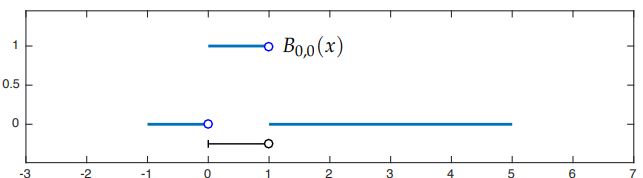
\includegraphics[width=0.5\columnwidth]{figures/KAN/BSplines1.png}
    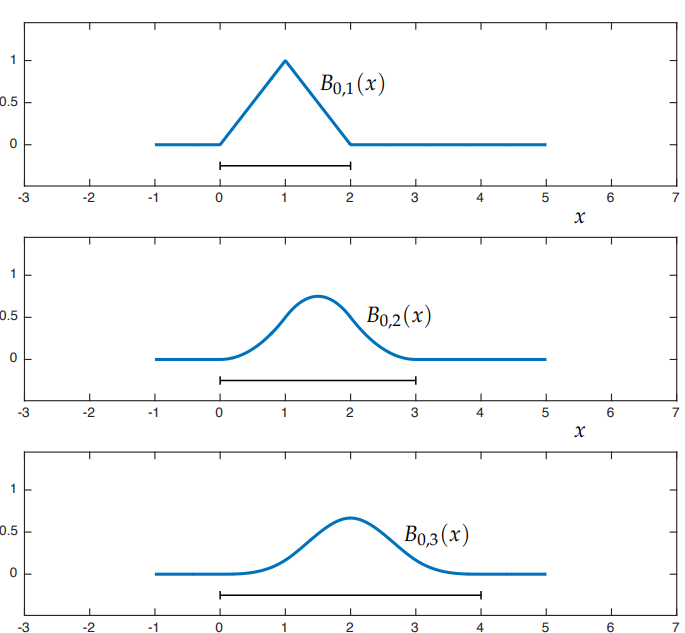
\includegraphics[width=0.5\columnwidth]{figures/KAN/BSplines2.png}
\end{figure}

\begin{figure}
    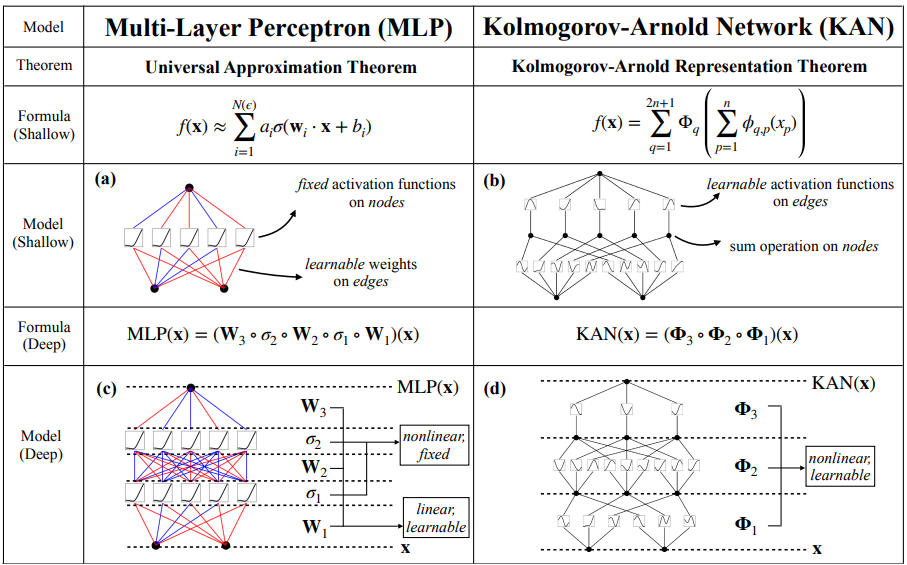
\includegraphics[width=\columnwidth]{figures/KAN/OverviewKANMLP.png}
\end{figure}
\begin{itemize}
    \item One main idea with the KANs is that they have better interpretability
    \item Aimed at math and physics applications
\end{itemize}
\subsection{Architecture}
\begin{itemize}
    \item Activation are on edges, not nodes, the nodes only do summation (no parameters)
    \item Non-linearity is applied on the edges before summing
\end{itemize}
	\section{Deep Reinforcement Learning 1 (Tabular Methods)}
\begin{figure}[!h]
    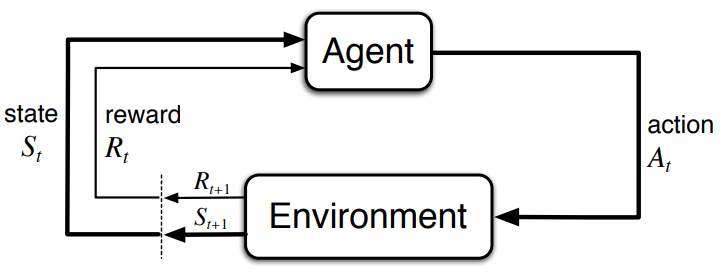
\includegraphics[width = 0.8\columnwidth]{figures/DeepReinforcementLearning1/EnvironmentAgent.png}
\end{figure}

Reinforcement Learning involves an agent interacting with an environment to learn decision-making. The agent:
\begin{itemize}
    \item Takes actions $A_t$ based on states $S_t$.
    \item Receives feedback in the form of rewards $R_t$.
    \item Learns to maximize cumulative rewards (return) $G_t$
\end{itemize}
cumulative reward or return (G):
\[
G_t = R_{t+1} + R_{t+2} + R_{t+3} + \dots + R_T
\]
Discounted return:
\[
G_t = R_{t+1} + \gamma R_{t+2} +\gamma^2 R_{t+3} + \dots = \sum_{k=0}^{\infty}\gamma^k R_{t+k+1}
\]
\begin{figure}[!h]
    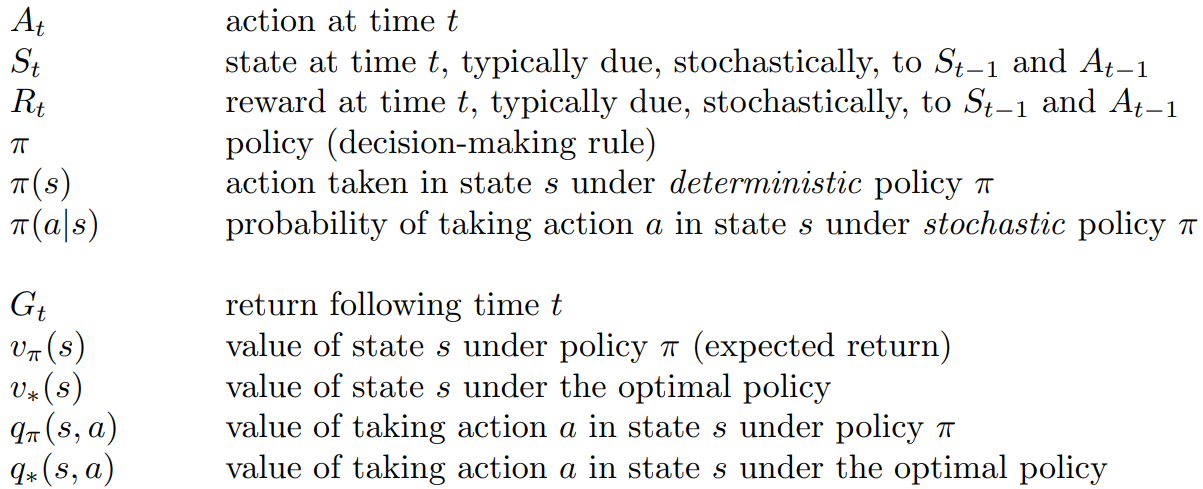
\includegraphics[width = \columnwidth]{figures/DeepReinforcementLearning1/OverviewNotation.png}
\end{figure}
\subsection{Formualtion of the Problem}
\begin{itemize}
    \item The actual value of an action \(a\) is the expected reward (which is not known)
    \[
    q_*(a) = \mathop{\mathbb{E}}[R_t|A_t = a]
    \]
    \item The estimated value of an action is called the (action-) value function \(Q_t(a)\) which we would like to be close to the true value
\end{itemize}
\subsubsection{Action-Value Mehtods}
\begin{itemize}
    \item Simple method(need to keep all rewards):
    \[
    Q_n = \frac{R_1 + R_2 +\dots + R_{n-1}}{n-1}
    \]
    \item Iterativ method:
    \[
    Q_{n+1} = Q_n + \frac{1}{n}(R_n - Q_n)
    \]
    \(R_n - Q_n\)(\(\left[Target- OldEstimation\right]\)) is like a Error.

\end{itemize}
This form
 \[\left[NewEstimation\leftarrow OldEstimation+StepSize\left[Error\right]
\right]\]
with different values for step and Error is used by many RL algorithm.
\subsection{Exploration vs Exploitation}
Exploitation:
\begin{itemize}
    \item Exploit current knowledge by taking  the action with the maximal estimated value
    \item Greedy action
\end{itemize}

Exploration:
\begin{itemize}
    \item Explore the value of other actions to get better estimates
    \item Non greedy actions
\end{itemize}
To balance Exploration and Exploitation:
\begin{itemize}
    \item \textbf{Exploitation:} With probability 1 - \(\epsilon\). Take greedy action with maximal \(Q_t(a)\)(greedy action)
    \item \textbf{Exploration:} With probability \(\epsilon\). Take any valid action with equal probability.
\end{itemize}
To use draw random variable in [0 .. 1].
Compare threshold with \(\epsilon\).
\begin{figure}[]
    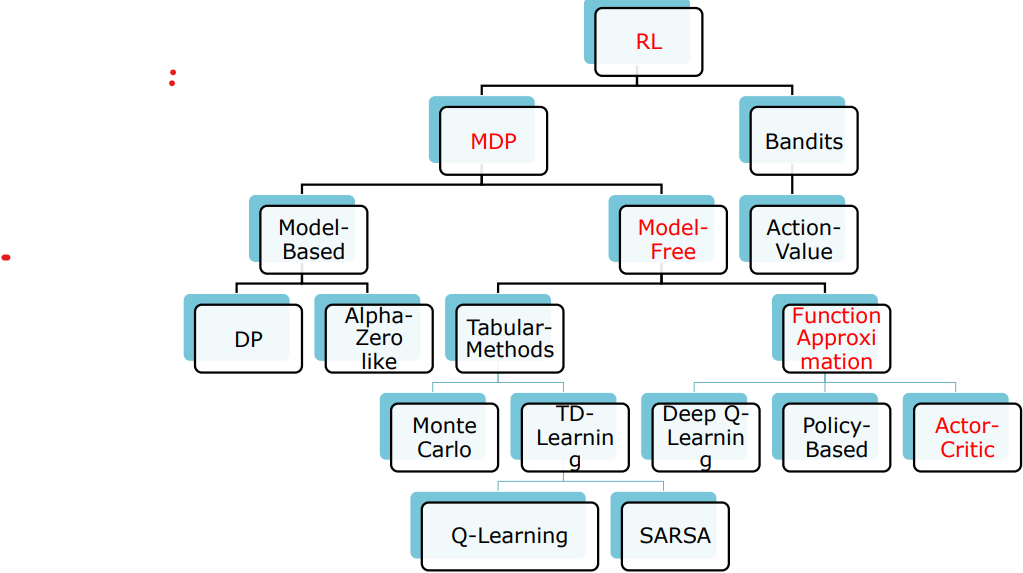
\includegraphics[width = \columnwidth]{figures/DeepReinforcementLearning1/RLOverview.png}
\end{figure}


\subsection{Mehtods Overview}

\subsection{Markov Decision Process (MDP)}
An MDP is defined by:
\begin{itemize}
    \item States $S$, actions $A$, and rewards $R$.
    \item Transition probabilities:
    \[
    p(s', r | s, a) = \Pr\{S_{t+1}=s', R_{t+1}=r | S_t=s, A_t=a\}
    \]
    \item Goal: Maximize the expected cumulative reward.
\end{itemize}

\subsection{Value Functions}
\subsubsection{State and Action-Value Functions}
\begin{itemize}
    \item State-value function under policy $\pi$:
    \[
    v_\pi(s) = \mathbb{E}_\pi[G_t | S_t = s]
    \]
    \item Action-value function under policy $\pi$:
    \[
    q_\pi(s, a) = \mathbb{E}_\pi[G_t | S_t = s, A_t = a]
    \]
\end{itemize}
\subsection{Policies}
A policy is a mapping from states to probabilities of selecting each possible action:
\[
\pi(a|s) = Pr\{A_t = a|S_t = s\}
\]
\subsubsection{Stochastic/Deterministic policies}
\begin{itemize}
    \item \textbf{Stochastic:} Different possible actions with different probabilities for each action. Example: rock, paper, scissor (1/3, 1/3, 1/3)
    \item \textbf{Deterministic:} Single action \(a\) is taken in a state \(s\).
\end{itemize}
\subsubsection{Bellman Equation}
For state-value function:
\[
v_\pi(s) = \sum_a \pi(a|s) \sum_{s', r} p(s', r | s, a) [r + \gamma v_\pi(s')]
\]
\subsection{Calculating the value function}
\begin{itemize}
    \item A solution to the value function for a policy can be found by solving the system of equations given by the Bellman equation for each state.
    \item If there are many states this system becomes large and computationally ineffective to calculate.
    \item We can solve it incrementally using Iterativ Mehtods (Dynammic Programming)
    \item However: Most often we do not have the Markov Decision Process given and have to explore the environment
\end{itemize}

\subsection{RL Algorithms: Value based methods}
\subsubsection{Monte-Carlo methods}
\begin{itemize}
    \item Monte-Carlo (MC) methods look at whole episodes and the average the complete results
    \item The task must be episodic
    \item Value estimations and policies are only changed \textbf{on the completion of an episode}
\end{itemize}

\subsubsection*{Monte Carlo Prediction}
\begin{itemize}
    \item We want to estimate \(v_\pi(s)\), the value of a state \(s\) under the policy \(\pi\).
    \item Given is a set of episodes.
    \item An episode might pass multiple times through\(s\), we will only consider it once, this is known as \textit{first-visit MC}.
    \item We average the retunrs of all episodes
\end{itemize}
\begin{figure}[!h]
    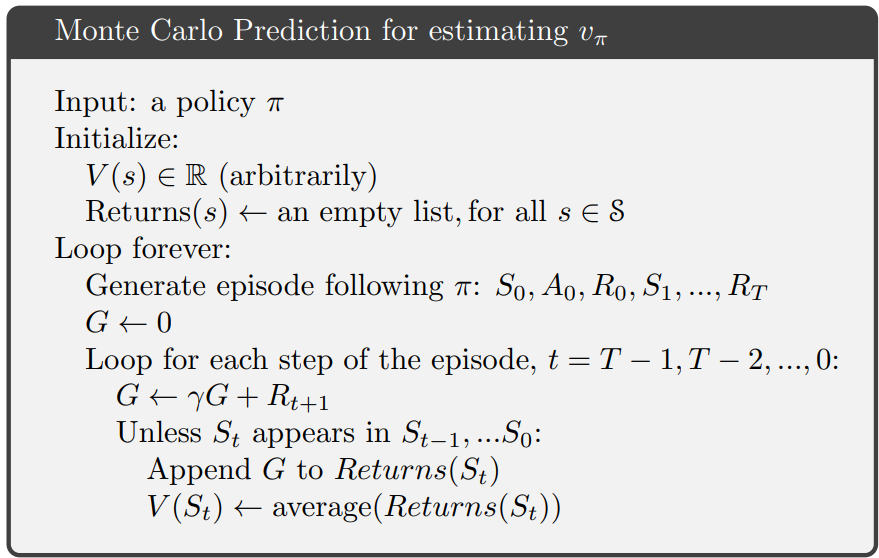
\includegraphics[width = \columnwidth]{figures/DeepReinforcementLearning1/MonteCarlo.png}
    \caption{Monte Carlo Prediction of the State-Value Function (first visit)}
\end{figure}

Intstead of averaging results, we would like an incremental calculation:
\[
    V(S_t) \leftarrow V(S_t) + \alpha[G_t - V(S_t)]
\]
If step size \(\alpha\) is \({1}/{n}\) its the same as averaging.

\subsubsection*{Policy Iteration:}
\begin{itemize}
    \item Knowing the state-value function will not help us to find a better policy, as we do not know which action will generate better returns
    \item Instead, we would like to predict the action-value function Q
    \item Given Q,we can find an improved policy by using greedy actions from Q 
    \item Using the new policy, we can predict its action-value function and repeat
    \item This is known as (generalized) policy-Iteration
\end{itemize}
\begin{figure}[!h]
    \centering
    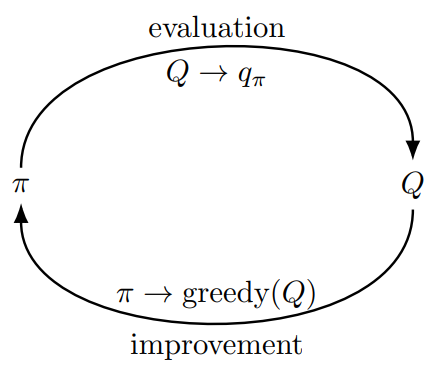
\includegraphics[width = 0.5\columnwidth]{figures/DeepReinforcementLearning1/PolicyIterationMonteCarlo.png}
\end{figure}

\subsubsection*{Exploration in MC}
\begin{itemize}
    \item We must maintain exploration to ensure that all state/action values are visited
    \item Out policy must be epsilon-soft:
    \item Each action in state must occur with a probability grater than zero
    \item 
\end{itemize}
\subsubsection{Temporal Difference (TD) Learning}
\begin{itemize}
    \item MC prediction with constant step size
    \[
    V(S_t) \leftarrow V(S_t) + \alpha[G_t - V(S_t)]
    \]

    \item TD methods make the update immediatly based on the estimates for the next state, which is just the application of the Bellman equation
    \[
    V(S_t) \leftarrow V(S_t) + \alpha[R_{t+1} + \gamma V(S_{t+1}) - V(S_t)]
    \]
\end{itemize}

\subsubsection*{SARSA (On-Policy TD Control)}
\begin{itemize}
    \item We use generalized policy iteration (GPI) for the control problem
    \item As in MC methods, we must balance exploration and exploitation 
    \item TD control methods generally learn an action-value function instead of a state-value function
    \item We look at the transition from (\textbf{S},\textbf{A}) with reward (\textbf{R}) to the next (\textbf{S},\textbf{A})(SARSA)
\end{itemize}
\[
Q(S_t, A_t) \leftarrow Q(S_t, A_t) + \alpha[R_{t+1} + \gamma Q(S_{t+1}, A_{t+1}) - Q(S_t, A_t)]
\]

\subsubsection*{Q-Learning (Off-Policy Control)}
\begin{itemize}
    \item SARSA uses teh Q-Values from the actual Action taken in the next step
    \item This action might not be the one, that maximizes the return
    \item While we cannot change the action taken, we can update the Action-Value using the best (or greedy) action from the next state, this is Q-Learning
\end{itemize}
\[
Q(S_t, A_t) \leftarrow Q(S_t, A_t) + \alpha[R_{t+1} + \gamma \max_a Q(S_{t+1}, a) - Q(S_t, A_t)]
\]
\begin{itemize}
    \item Q-Learning directly tries to approximate the optimal action-value function
    \item It uses a \textbf{soft policy} to determine which actions to take during the episode and the \textbf{greedy policy} to update the action-value estimates
    \item It is called a \textbf{off-policy} algorithm
\end{itemize}
\subsubsection*{Adaptaion}
\begin{itemize}
    \item \textbf{n-Step TD Prediction:} Instead of taking one step and then update the Q-Values we could take 2 or more Steps
    \item \textbf{Lamda-Returns:} Lamda-returns use a weighted sum of all the returns for the estimation
    \[
    G_t^\lambda = (1-\lambda)\sum_{n=1}^{\infty}\lambda^{n-1}G_{t:t+n}
    \]
\end{itemize}
\subsubsection{Summary value based methods}
\textbf{Monte Carlo Estimate:}
\begin{itemize}
    \item Calulate from one episode, estimate is sum of reward
    \item Multiple episode might go through the same state, the MC estimate is the average of those
    \item Estimate have \textbf{high variance}, as the estimates involve many (random) processes and decision along the entire episode
    \item They are \textbf{unbiased}
\end{itemize}
\subsubsection*{TD Estimate:}
\begin{itemize}
    \item A single reward is used and the estimate of the expected return from the next state (the estimate is using another estimate)
    \item Estimates of the next state will not be accurate early in the training
    \item Low variance, as you only depend on the next Steps
    \item Biased, because the estimate depends on the estimate of the next step, which might be inaccurate
\end{itemize}





	\section{Deep Reinforcement Learning 2 (Function Approximation)}
\begin{itemize}
    \item We want to approximate a state-values or the state-action-values by function that is parametrized by some paramer \textbf{w}.
    \[
    \hat{v}(s,\boldsymbol{w}) \approx v_\pi(s)
    \]
    \[
    \hat{q}(s,a,\boldsymbol{w}) \approx q_\pi(s,a)
    \]
    \item The dimensionality \(d\) of \textbf{w} will generally be much lower than the dimensionality of the state space
    \[
    d \ll |S|
    \]
    \item While there are many possibilities for function approximation, we will concentrate on \textbf{neural networks}
\end{itemize}
\subsubsection*{Prediction Objectiv}
As an objectiv, we would like to learn to approximate the value function at each state, so that the following error function is minimized:
\[
\left[v_\pi(s)-\hat{v}(s,\boldsymbol{w})\right]^2
\]
However, an update to one state, will affect the other state.
We want to introduce a function \(\mu(s)\) that measures how important each error is and then minimize the mean weighted error between the value function and its approximation.
\[
\overline{VE}(\boldsymbol{w}) = \sum_{s\in S}^{}\mu(s)\left[v_\pi(s)-\hat{v}(s,\boldsymbol{w})\right]^2
\]
(In practice,this just means that our samples are not distributed equally over all states.)
\subsection{Stochastic gradient descent}
\begin{itemize}
    \item Let us assume that in each step we observe a state \(s\) and its (true) value under the policy.
    \item We can use stochastic gradient-descent (SGD) to minimize the error in the observed examples
\end{itemize}
\begin{align*}
    \boldsymbol{w}_{t+1} &= \boldsymbol{w}_t - \frac{1}{2}\alpha\nabla\left[v_\pi(s)-\hat{v}(s,\boldsymbol{w})\right]^2\\
    &= \boldsymbol{w}_t + \alpha\left[v_\pi(s)-\hat{v}(s,\boldsymbol{w})\right]\nabla\hat{v}(S_t,\boldsymbol{w}_t)
\end{align*}
\begin{figure}[h]
    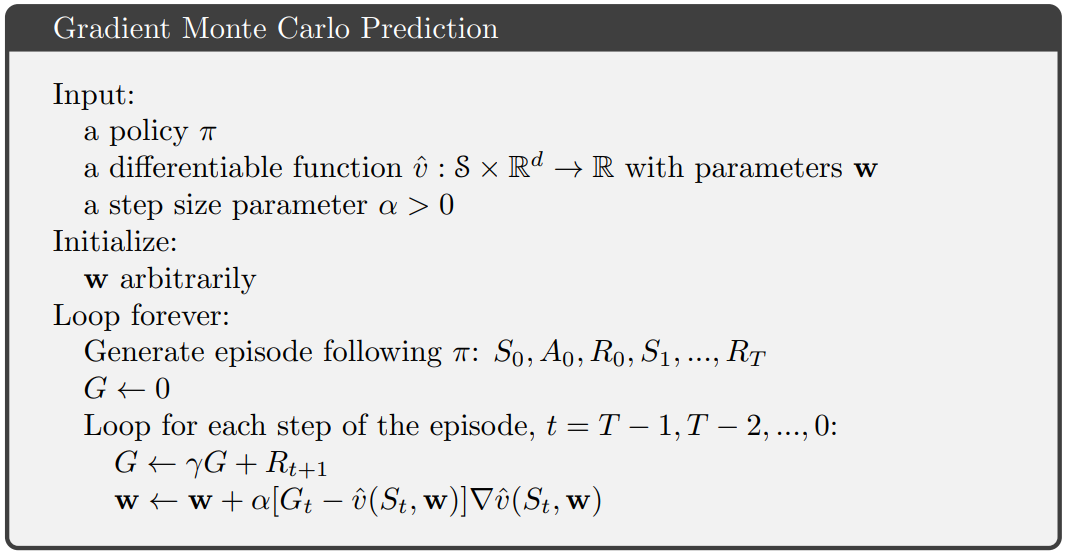
\includegraphics[width = \columnwidth]{figures/DeepReinforcementLearning2/GDMonteCarlo.png}
\end{figure}

\subsection{Deep Q-Learning}
\begin{figure}[!h]
    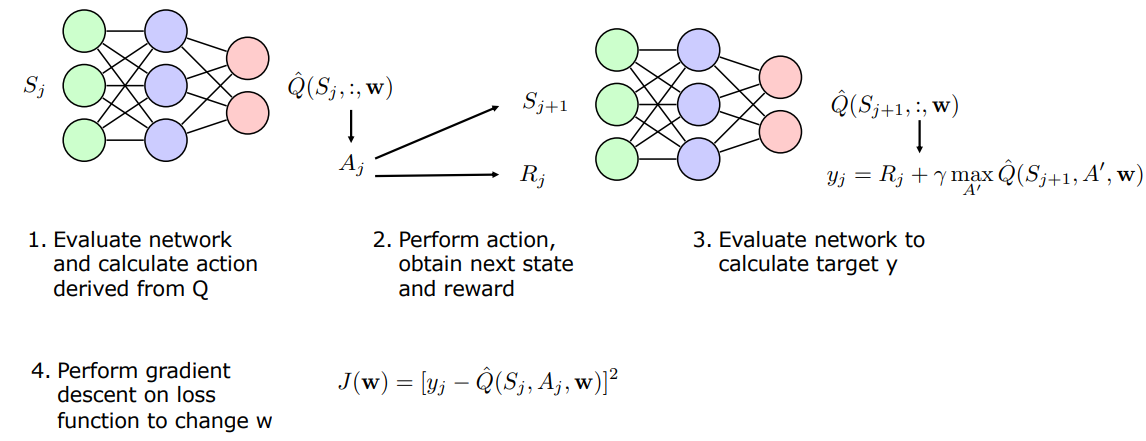
\includegraphics[width = \columnwidth]{figures/DeepReinforcementLearning2/BasicDeepQLearning.png}
\end{figure}
Use a neural network to approximate the Q-Function.
As multiple actions are needed to evaluate, multiple passes through the network are required.

A better approach is to use a neural network with inputs \(s\) to calculate the action-value function for all the actions simultaneously.
The output is a vector with a different q values for a given state.


\subsubsection{Problem: Moving Target}
\begin{itemize}
    \item As the calculation of the target function also depends on \textbf{w}, it will also be changed after a gradient step
    \item The target moves with every update to \textbf{w} while we are trying to approximate it.
    \item It is better to let the target remain stable, for this, another set of weights \(\boldsymbol{w}^-\) can be used that are updated after a few step.
\end{itemize}

\subsection{Experience Replay}
\begin{itemize}
    \item It is not efficient to update the network after one step
    \item Futhermore, a sample should be used more than once, similar to supervised learning, where we go over the data set multiple times
\end{itemize}
The \textbf{experience} at each time step is stored into a data set
\begin{align*}
    e_t &= (s_t, a_t, r_t, s_{t+1})\\
    D &= e_1, \dots, e_N
\end{align*}
\begin{itemize}
    \item A fixed size buffer is used that overwrites the oldest experience
    \item Training data then \textbf{sampled} from the data set
\end{itemize}
\begin{figure}[!h]
    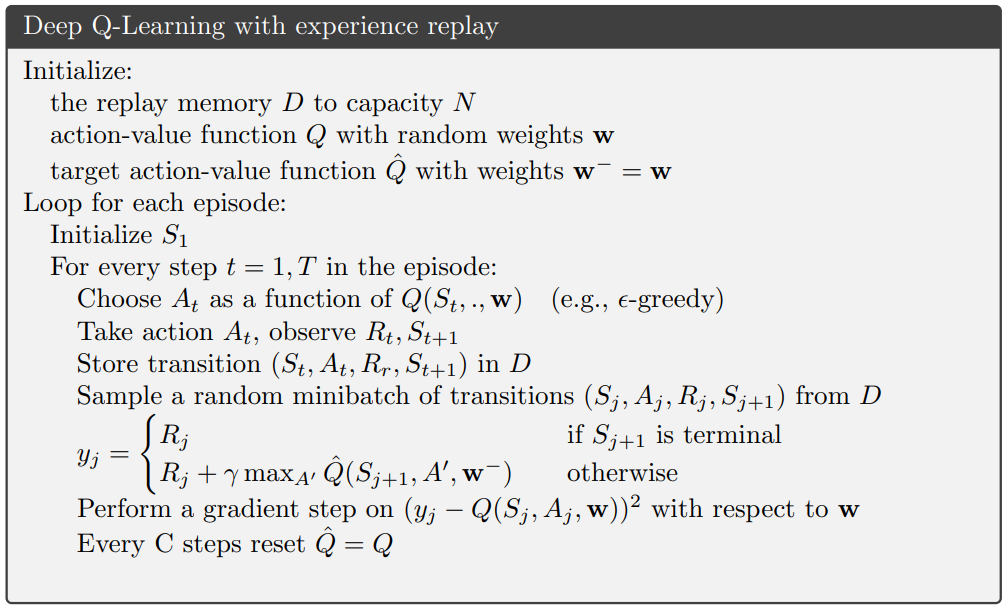
\includegraphics[width = \columnwidth]{figures/DeepReinforcementLearning2/DeepQLearningExperienceReplay.png}
\end{figure}

\subsection{Optimizing Deep Q-Learning}
Training for Deep Q-Learning is often difficult; several further concepts have been developed to make training easier:
\begin{itemize}
    \item Prioritized Experience Replay
    \item Double Q-Learning
    \item Dueling Networks
    \item Multi-step bootstrap targets
    \item Distributional DQN
    \item Noisy DQN
    \item Options of target weights update
\end{itemize}

\subsection{Policy Based Methods}
\begin{itemize}
    \item So far, all methods have been \textit{action-value methods}
    \item Policies were only calculated from those action-value estimates (using GPI)
    \item We now turn to methods that directly learn a parmetrized policy
    \[
    \pi(a|s,\boldsymbol{\theta}) = Pr\left\{A_t = a|S_t = s,\boldsymbol{\theta}_t = \boldsymbol{\theta}\right\}
    \]
    where \(\boldsymbol{\theta}\) are the parameters (weights) of the function that approximates the policy
\end{itemize}
\subsubsection*{Goal: Maximize Performance}
We want to change the weights, so that the return is maximized.
There are different algorithms to do that:
\begin{itemize}
    \item "Hill Climbing"
    \item Gradient Ascent
\end{itemize}

\subsubsection*{Policy Optimization with Hill Climbing}
Idea:
\begin{enumerate}
    \item Initialize weights for the function approximation arbitrarily
    \item Calculate the return \(G\) of an episode using the weights
    \item Change the weights slightly (add random noise)
    \item Calculate the return \(G\) using the new weights
    \item If return is larger: keep the new weights, decrease noise
    \item Otherwise: restore old weights, increase noise
    \item Continue with step 3
\end{enumerate}

\subsubsection{Why Policy-Based Methods}
\begin{itemize}
    \item While the goal of RL has been defiend is to maximize return \dots
    \item \dots we are not intrested in the actual value function, but
    \item \dots the \textbf{goal is to find the policy}
    \item Policy-based methods can learn true \textbf{stochastic policies}, this is different from epsilon greedy methods which add randomness just exploration
    \item Aliased states: States that look similar (same observation) but are actually different are difficult to handle with deterministic policies
    \item Finding the optimal action in values-based methods is difficult for continuous action spaces
\end{itemize}

\subsection{Policy Gradient Methods}
\begin{itemize}
    \item \textbf{Policy-based methods:} Search for optimal policy
    \item \textbf{Policy gradient methods:} Use \textbf{gradient ascent} to find the best parameters (Requires the approximation function to be differentiable)
    \[
    \boldsymbol{\theta}_{t+1} = \boldsymbol{\theta} + \alpha \widehat{\nabla J(\boldsymbol{\theta})}
    \]
    where
    \[
    \widehat{\nabla J(\boldsymbol{\theta})}
    \]
    is a stochastic estimate of the gradient of the performance measure.
\end{itemize}

\subsubsection*{Constrains for the policy}
The policy should be a probability function over the different actions and must use exploration, therefor:
\begin{itemize}
    \item The probability of any action should be greater than 0:
    \[
    \pi(a|s,\boldsymbol{\theta}) > 0, \text{for all } a \in A,s \in S
    \]
    \item The sum of all probabilities must be 1:
    \[
    \sum_{a}^{}\pi(a|s,\boldsymbol{\theta}) = 1, \text{for all } s \in S
    \]
    \item Use action-preferences and softmax:
    \[
    h(s,a,\mathbf{\theta})\in\mathbb{R} \qquad \pi(a|s,\boldsymbol{\theta}) = \frac{e^{h(s,a,\boldsymbol{\theta})}}{\sum_{b}^{e^{h(s,b,\boldsymbol{\theta})}}}
    \]
\end{itemize}

\subsubsection*{Episodic case}
\begin{itemize}
    \item Goal: optimize the total return from a (particular) state
    \[
    J(\boldsymbol{\theta}) = v_{\pi\boldsymbol{\theta}}(s_0)
    \]
    \item Problem: v depends on action selection and state distribution
    \item Policy gradient theorem:
    \[
    \nabla J({\boldsymbol{\theta}})\propto \sum_{s}^{}\mu(s)\sum_{a}^{}q_\pi(s,a)\nabla\pi(a|s,\boldsymbol{\theta})
    \]
\end{itemize}

\subsubsection*{REINFORCE: Monte Carlo Policy Gradient}
\begin{itemize}
    \item Update the weights according to:
    \begin{align*}
        \boldsymbol{\theta}_{t+1} &= \boldsymbol{\theta} + \alpha G_t\frac{\nabla\pi(A_t|S_t,\boldsymbol{\theta})}{\pi(A_t|S_t,\boldsymbol{\theta})}\\
        &= \boldsymbol{\theta} + \alpha G_t\nabla ln\pi(A_t|S_t, \boldsymbol{\theta})
    \end{align*}
    \item The second line can be derived from
    \[
    \nabla ln(f(x)) = \frac{\nabla f(x)}{f(x)}
    \]
    \item This is gradient \textbf{ascent}, as we want to maximize the return
\end{itemize}
\subsubsection*{How policy gradient works}
\begin{itemize}
    \item After the episode is complete, the policy gradient algorithm will look at each state and consider the selected action.
    \item If the return G was to high, it will make the action more likely
    \item If the return was low, it will reduce the probability
\end{itemize}

\subsubsection*{Problems with REINFORCE}
Policy Gradient is Noisy!
\begin{itemize}
    \item Gradient should be over millions episodes or trajectories (truncated episodes)
    \item But we typically only use one trajectory
    \item We should generate a number of trajectories, and calculate the trajectory from them 
    \item We can then also reduce noise by calculating the mean and standard deviation of the samples by reward normalization, this is called batch normalization
\end{itemize}

\subsubsection*{Baseline}
A "trick" for faster convergence and less variance is to subtract a baseline from the q values, where the baseline can be any function that does not depend on the action
\[
\nabla J({\boldsymbol{\theta}})\propto \sum_{s}^{}\mu(s)\sum_{a}^{}(q_\pi(s,a)-b(s))\nabla\pi(a|s,\boldsymbol{\theta})
\]
\[
    \boldsymbol{\theta}_{t+1} = \boldsymbol{\theta} + \alpha (G_t-b(S_t))\frac{\nabla\pi(A_t|S_t,\boldsymbol{\theta})}{\pi(A_t|S_t,\boldsymbol{\theta})}
\]
\begin{itemize}
    \item A natural choice for b, is to estimate a state value
    \[
    \hat{v}(S_t,\boldsymbol{w})
    \]
    \item where the weights would also be learned using the Monte-Carlo method
    \item The function is not dependent on the policy parametrization, so the gradient remains the same
    \item The difference between q and v is also called the \textit{advantage} function:
    \[
    q(s,a) - v(s)
    \]
\end{itemize}

\subsubsection*{Why does this baseline help?}
\begin{itemize}
    \item The current policy is used to sample actions, while the policy is also update from observations from the same actions.
    \item This creates an exploration-exploitation dilemma
    \item With a value baseline, the aggressiveness of the updates is reduced
\end{itemize}
\subsubsection{Summary Policy Gradient Methods}
Advantages:
\begin{itemize}
    \item Often better convergence properties
    \item Effective in high dimensional or continuous action spaces
    \item Can learn stochastic policies
\end{itemize}
Disadvantages:
\begin{itemize}
    \item Typically converge to local rather than global optimum
    \item Evaluating a policy can be inefficient and high variance
\end{itemize}
\subsubsection*{More on policy gradient Methods}
\begin{itemize}
    \item This was the \textit{vanilla} policy gradient method
    \item There are variations regarding the update and the sampling that make the methods more stable and faster to converge
    \item These are the Trust Region Policy Optimization (TRPO) and the Proximal Policy Gradient (PPO) methods
\end{itemize}

\subsection{Actor-Critic Methods}
1-step Policy Gradient Method with Critic
\begin{itemize}
    \item We would like to implement a 1-step (or n-step) method like TD(0) for the policy
    \item However, we then need a \textbf{value} function, so we can replace the full return in REINFORCE with the 1-step return:
    \begin{align*}
        \boldsymbol{\theta}_{t+1} &= \boldsymbol{\theta}_t + \alpha(R_t + \gamma\hat{v}(S_{t+1},\boldsymbol{w})-\hat{v}(S_t,\boldsymbol{w}))\nabla \text{ln}\pi(A_t|S_t,\boldsymbol{\theta}_t)\\
        &= \boldsymbol{\theta}_t + \alpha\delta_t\nabla \text{ln}\pi(A_t|S_t,\boldsymbol{\theta}_t)
    \end{align*}
    \item The policy is called the \textit{actor}, the value function the \textit{critic}
    \item The value function approximation can be calculated as in deep Q-Learning
\end{itemize}
\begin{figure}[!h]
    \centering
    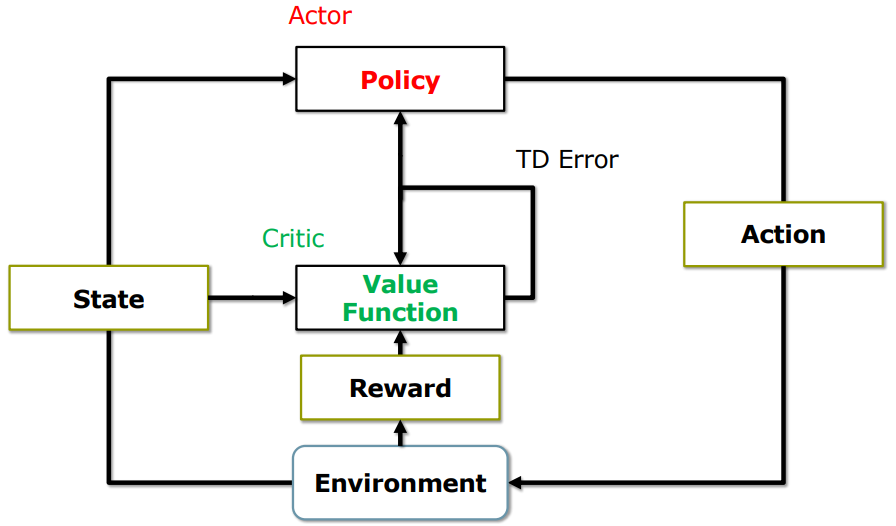
\includegraphics[width = \columnwidth]{figures/DeepReinforcementLearning2/ActorCritic.png}
\end{figure}

\subsection{Overview: Value and Policy based Methods}
Value Based:
\begin{itemize}
    \item Learnt Value Function
    \item Implicit Policy (e.g. epsilon greedy)
\end{itemize}
Policy Based:
\begin{itemize}
    \item No Value Function
    \item Learnt Policy
\end{itemize}
Actor-Critic
\begin{itemize}
    \item Learnt Value Function
    \item Learnt Policy
\end{itemize}

\subsubsection*{Example: How to play tennis?}
Policy based(REINFORCE):
\begin{itemize}
    \item Play matches
    \item Think about the matches that you won and lost, and do more of the actions you did in the won matches and less of those in the lost matches
\end{itemize}
Value based
\begin{itemize}
    \item You guess what the score will be like (during the match) and select actions that maximize the score
    \item Guesses get better, resulting in better performance
    \item but guesses can be wrong(biased, prone to over or underestimate)
\end{itemize}
Actor-Critic based:
\begin{itemize}
    \item Combine both approaches
    \item Actor Critic methods are more stable than value-based agents and need fewer samples than policy-based approaches
\end{itemize}
\subsubsection*{Different Actor-Critic/Policy Gradient Methods}
There are different choices for the value of \(\psi\) in the expression for the gradient:
\[
\psi \nabla_{\boldsymbol{\theta}} \text{ln}\pi(A_t|S_t,\boldsymbol{\theta})
\]
\begin{table}[!h]
    \begin{tabular}{lr}
    \(\psi = G\)    &  Return from episode\\
    \(\psi = Q(A_t,S_t)\)     &  Action-value function\\
    \(\psi = A(A_t,S_t)\)     &  Advantage function\\
    \(\psi = r_t + V(S')-V(S)\)     & TD(0) residual
    \end{tabular}
\end{table}
	% \input{Sections/04_Interprozesskommunikation}
	% \input{Sections/06_Deadlocks_PriorityInversion}
	% \input{Sections/07_Scheduling}
	% \input{Sections/08_Speicherhierarchie}
	% \input{Sections/10_Speicherverwaltung}
	
	% \input{Sections/99_CodeBeispiele}

\end{document}
